\section{Approfondimento obiettivi} \label{sec:obiettivi_approfondimento}
Abbiamo già visto (vedi \nameref{sec:obiettivo}) che un obiettivo può essere a \textbf{focale fissa} (in inglese \textit{prime}) o \textbf{zoom} (in inglese rimane \textit{zoom}).

Solitamente non si soliti distinguere le lenti in base al fatto che siano fisse o zoom, ma si guardano la focale (i.e. la lunghezza), il diaframma e lo scopo per cui la lente è pensata.

Vediamo ora un piccolo approfondimento su quello che abbiamo già visto sulle lenti, e a seguire alcune categorie di lenti, non differenziate in base alla lunghezza focale, ma allo scopo per cui sono state pensate.

Approfondimenti:
    \begin{itemize}
        \item[-] \nameref{subsec:primevszoom}
        \item[-] \nameref{subsec:suigrandandoli}
        \item[-] \nameref{subsec:sullestandard}
        \item[-] \nameref{subsec:suitele}
        \item[-] \nameref{subsec:innesto} 
    \end{itemize}

Lenti per scopo:
    \begin{itemize}
        \item[-] \nameref{subsec:lentimacro}
        \item[-] \nameref{subsec:lentidecentrabili}
        \item[-] \nameref{subsec:lenticatadiottriche}
        \item[-] \nameref{subsec:lentipinhole}
    \end{itemize}


\subsection{Innesto} \label{subsec:innesto}
Le macchine fotografiche hanno obiettivi interscambiabili, quindi corpi macchina e obiettivi sono due corpi separati che possono essere scambiati.

Non esiste un singolo innesto, bensì ogni azienda che produce fotocamere ha i propri innesti che monta sulle proprie fotocamere.

Si possono usare lenti pensate per un diverso innesto? Sì, esistono degli anelli adattatori pensati con questo preciso scopo; bisogna però tenere a mente che se gli obiettivi non sono stati pensati per essere montati sull'innesto della nostra macchinetta possono esserci problemi di compatibilità.
Ad esempio la messa a fuoco automatica può dare problemi.

Negli innesti si trovano solitamente dei piccoli pin dorati, che si connettono con dei pin simili che si trovano anche sugli obiettivi, in questo modo corpo macchina e obiettivo possono comunicare.
Le informazioni che si passano riguardano principalmente i settaggi per l'esposizione e per la messa a fuoco automatica. Su obiettivi completamente manuali (i.e. messa a fuoco e ghiera per regolare il diaframma manuali) mancano i pin, in questo modo non possono comunicare con il corpo macchina, che non avrà accesso ad alcune informazioni, come ad esempio l'apertura del diaframma.

Ogni innesto ha un valore fisso di \textbf{tiraggio}, ovvero la distanza tra il sensore (o la pellicola) e il bocchettone d'innesto per gli obiettivi.
Serve conoscere il tiraggio della propria macchinetta? Solitamente no, ma diventa importante tenerne conto nel momento in cui vogliamo montare un obiettivo con un innesto diverso usando un adattatore.

Esempio pratico: l'innesto che usa oggi Canon sulle reflex si chiama EF, per anni (dal 1971 al 2003) ha usato un attacco per le fotocamere analogiche chiamato FD.
A causa di un problema di tiraggio, se si monta un obiettivo FD su una fotocamera EF, la messa a fuoco è completamente scalibrata e l'obiettivo è quasi inutilizzabile.
Esiste una soluzione, ci sono anelli adattatori che non si limitano a fare da tramite tra i due attacchi, ma hanno una lente che corregge questo problema; il difetto di questi anelli è che costano molto e la lente aggiunta dell'anello impatta sulla qualità della foto (più vetro deve attraversare la luce e peggio arriva sul sensore, come risultato le immagini risultano più morbide, ovvero meno nitide).

\subsection{Focale fissa vs Zoom} \label{subsec:primevszoom}
È bene capire che, sebbene interessi la focale e non se l'obiettivo può zoommare o meno, in molti casi è preferibile usare una lente fissa, perché?

Le lenti zoom hanno la comodità di avere più focali in una, permettono di fare diversi tipi di fotografia senza cambiare obiettivo. Hanno però tanti difetti, che in certi casi possono essere ignorati, ma è comunque importante capire cosa ci offrono le lenti zoom per fare un acquisto più oculato. Teniamo a mente che le lenti zoom sono molto più complicate delle lenti fisse, da qui derivano tutti i problemi che stiamo per vedere.

Il primo difetto, più evidente, delle lenti zoom è che, zoommando, il diaframma si chiude. Come facciamo a sapere quanto si chiude? Ce lo dice il nome della lente.\newline
Riprendiamo come esempio il \lens{18-55}{3.5-5.6}; con la lente a 18mm possiamo tenere il diaframma aperto fino ad un massimo di $f/3.5$, man mano che zoommiamo si chiude sempre di più, raggiunti i 55mm l'apertura massima diventa $f5.6$. Esistono lenti zoom che non chiudono il diaframma, ma sono lenti di fascia alta con prezzi certamente meno accessibili.

Il diaframma è spesso inotre un po' più chiuso, a meno di andare su modelli di fascia alta, raramente si trovano lenti zoom con un diaframma che apre oltre $f/3.5$.

Le lenti zoom hanno anche più elementi al loro interno, e tendono ad essere più grandi, pesanti, e quindi costose.
Inoltre tendono a dare foto con una qualità inferiore (i.e. meno \textit{nitide}) rispetto alle lenti fisse; questo però era vero specialmente tanti anni fa, oggi la differenza si è molto assottigliata e le lenti zoom danno risultati più che buoni.
Bisogna anche precisare che la differenza di nitidezza c'è ma non sempre, si possono tranquillamente prendere una lente fissa di fascia bassa e una lente zoom di fascia alta; la lente zoom, in fatto di nitidezza può tranquillamente battere la lente fissa, dipende da lente a lente.

Tutti i problemi di cui sopra sono così proibitivi? Dipende, ma in generale no, specialmente per un uso più amatoriale vanno più che bene. Specialmente se non si hanno intenzioni troppo serie con la macchinetta si può prendere una sola lente zoom per portarsela in giro e fare tutti gli scatti che servono, senza portarsi dietro diverse lenti fisse, che occupano spazio, pesano e vanno ogni volta cambiate.

%\begin{figure}[H]
%    \centering
%        \begin{subfigure}{0.33\linewidth}
%            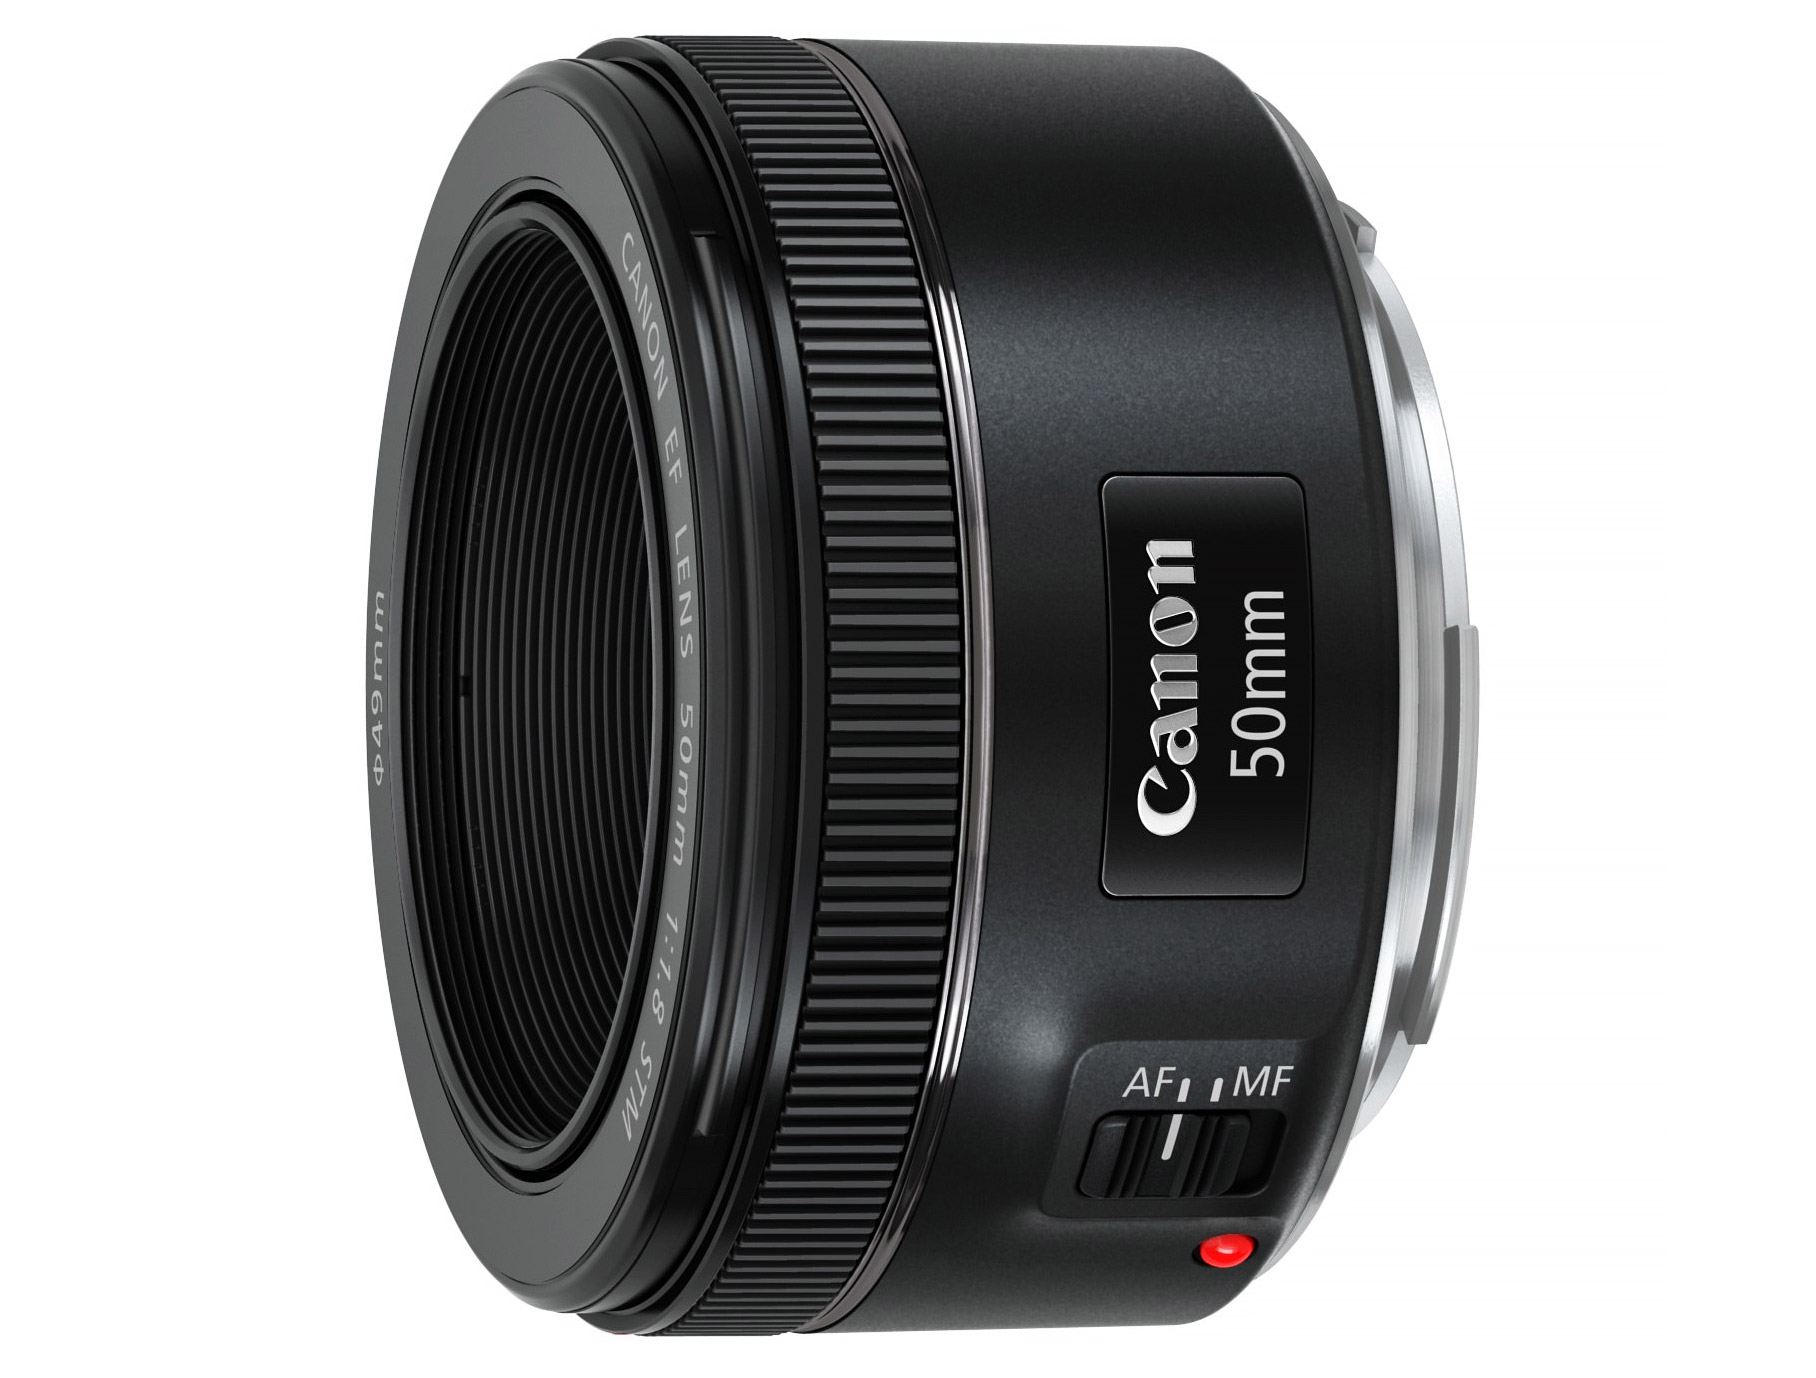
\includegraphics[width=\linewidth]{obiettivo_canon_50.jpg}
%            \caption{Canon 50mm $f/1.8$}
%        \end{subfigure}
%    %\hfil
%        \begin{subfigure}{0.33\linewidth}
%            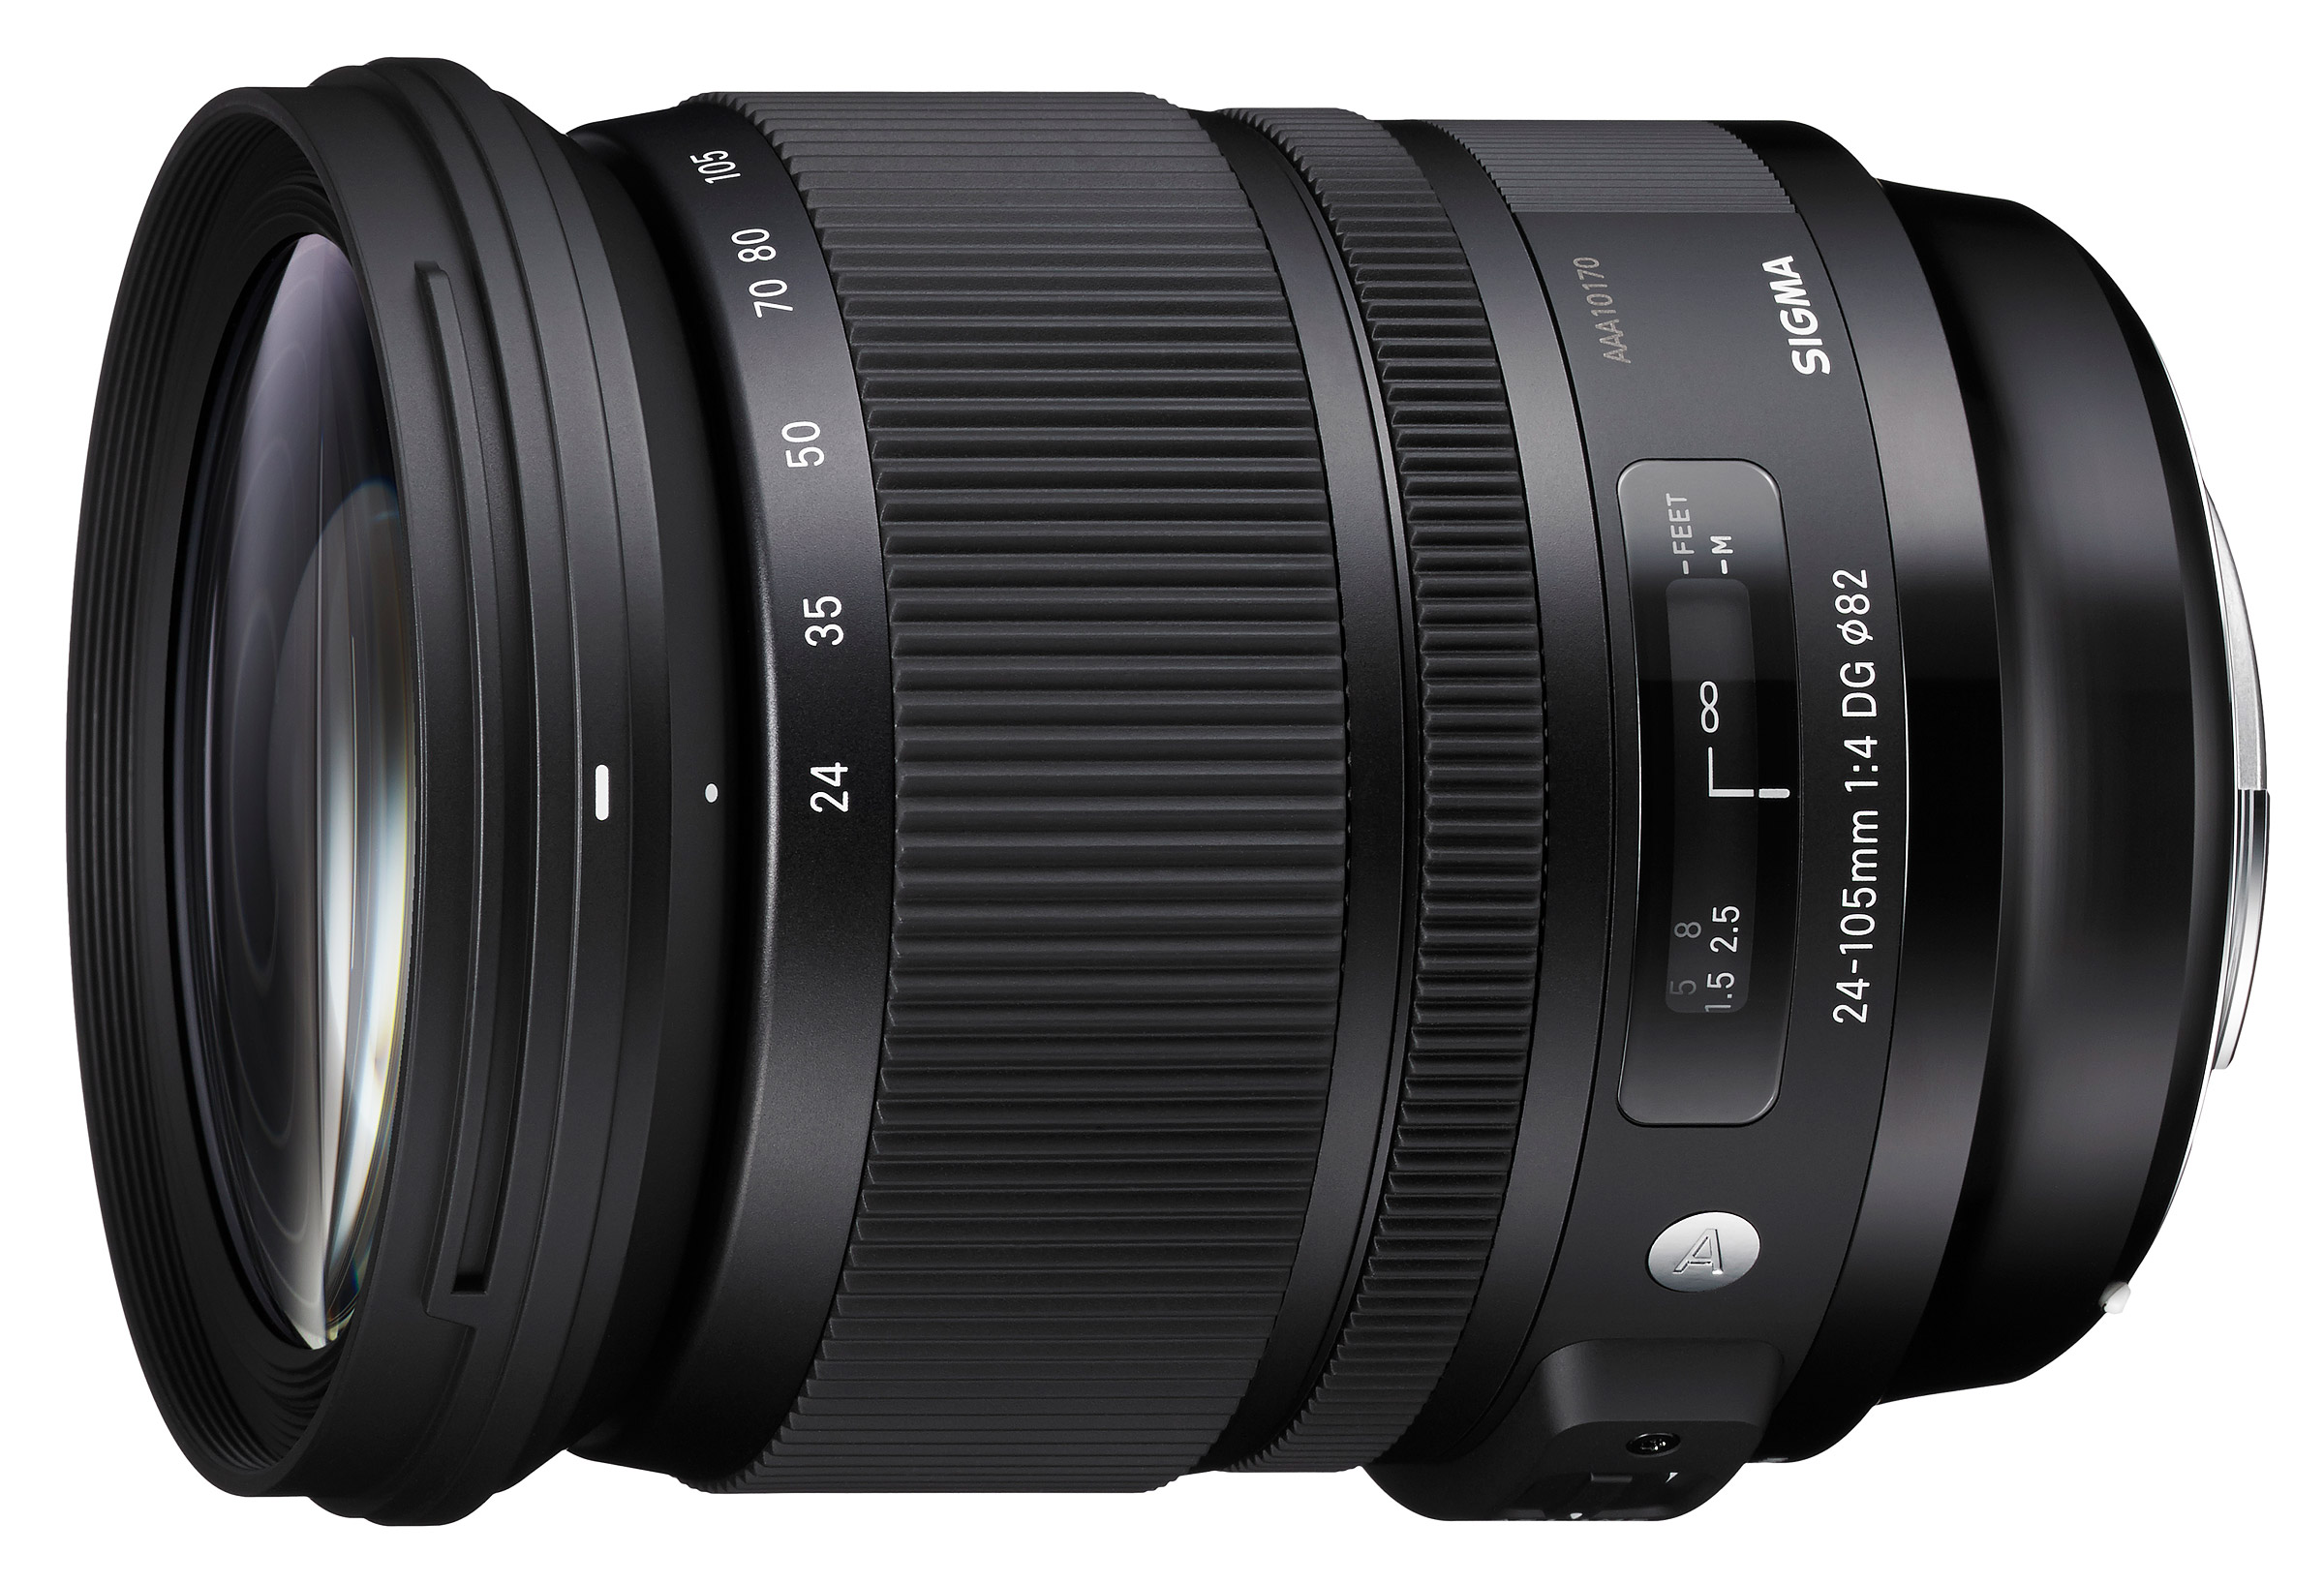
\includegraphics[width=\linewidth]{obiettivo_sigma_24_105.jpg}
%            \caption{Sigma 24-105mm $f/4$\\DG OS HSM Art}
%        \end{subfigure}
%
%    %\caption{2 x 3 grid of images}
%    \label{fig:lens_zoomvsprime}
%\end{figure}

\subsection{Sui grandangoli} \label{subsec:suigrandandoli}
I grandandoli sono lenti con ampi angoli di campo, che mostrano una buona fetta di scena. I grandangoli più estremi sono detti \textbf{fisheye}.

Un grandangolo tende ad aumentare le distanze tra gli oggetti; man mano che ci si avvicina al centro dell'immagine gli elementi che la compongono sembrano sempre più lontani e piccoli.
Il boke è spesso molto limitato o inestistente, permettono di mettere a fuoco facilmente tutta la scena.

La distorsione delle immagini che esce fuori da queste lenti viene detta \textit{barrel distorion}, \textit{a barile}, ovvero l'immagine diventa un po' "bombata".


\subsection{Sulle lenti standard} \label{subsec:sullestandard}
Restituiscono immagine poco distorte e molto vicine alla realtà, così come possiamo osservarle con i nostri occhi. Sono lenti molto versatili, molto apprezzate per i ritratti.

Due focali molto usate per la ritrattistica sono il 50mm e l'85mm, non distorcono molto l'immagine e offrono generalmente un boke gradevole.


\subsection{Sui teleobiettivi} \label{subsec:suitele}
A grandi linee sui teleobiettivi si può dire tutto l'opposto di quello che si è detto sui grandangoli.

Le distanze tra gli oggetti vengono schiacciate, oggetti che, in profondità, sono distante decine o addirittura centinaia di metri sembrano quasi stare vicini, sullo stesso piano.\newline
Il boke è molto accentuato, specialmente se cerchiamo di fotografare soggetti non molto distanti da noi.

Se dai grandangoli esce fuori una distorsione bombata, qui è il contrario, viene detta \textit{a cuscino}; è come se ci fosse un peso al centro dell'immagine che tira tutto a sé.


\subsection{Macro} \label{subsec:lentimacro}
Sono lenti pensate per la fotografia \textit{macro}, cioè permettono di metterre a fuoco soggetti molto vicini alla lente.

Non hanno una lunghezza precisa, ci sono lenti macro più o meno lunghe, ma spesso hanno focali sui 60mm o più.\newline
Nella fotografia macro è importantissimo avere tanta luce e quanta più nitidezza possibile, ne viene che le lenti macro sono sempre lenti fisse con un diaframma molto aperto.

Un obiettivo si definisce macro quando ha un \textbf{rapporto di ingrandimento} di almeno \textbf{1:1}. Cosa significa?
Più mettiamo a fuoco un soggetto vicino alla lente, e più questo soggetto appare grande sul sensore. Avere un rapporto 1:1 significa che un oggetto compare a grandezza naturale sul sensore.

Se ad esempio fotografiamo un insetto grande 1cm con un rapporto 1:1, l'insetto occuperà sul sensore esattamente 1cm.

Esistono lenti più spinte con rapporti di ingrandimento maggiori; un esempio è il Canon \lens{65}{2.8}, che raggiunge un rapporto di 5:1. Con 5:1 se fotografassimo l'insetto di prima, grande 1cm, questo occuperebbe uno spazio di 5cm sul sensore; i.e. viene ingrandito 5 volte.

Esistono tanti obiettivi che non sono esattamente macro, ma vengono venduti con la dicitura "Macro 1:2". Significa che raggiungono un rapporto di ingrandimento di 1:2, ovvero un soggetto non viene rappresentato a grandezza naturale sul sensore ma è la metà della grandezza naturale. Non sono vere e proprie lenti macro, ma permettono comuqnue di fare fotografie macro, da molto vicino, senza essere troppo spinte. Questi obiettivi possono essere usati per fare qualche primo tentativo di fotografia macro, senza spendere centinaia di euro per una lente dedicata alla macro fotografia se non si è ancora convinti.


\subsection{Decentrabili} \label{subsec:lentidecentrabili}
Sono ottiche molto particolari, pensate per la fotografia d'architettura. In inglese vengono chiamate \textit{tilt-shift}.

Solitamente non hanno focali troppo spinte, si trova un po' di tutto dai 17mm ai 135mm circa.

La particolarità sta nel poter fisicamente muovere l'ottica, facendo due movimenti:
\begin{itemize}
    \item[-] \textbf{Decentramento}
    \item[-] \textbf{Basculaggio}
\end{itemize}

Il \textbf{decentramento} (o \textit{shift}) muove la lente in parallelo a destra e sinistra davanti il sensore; serve a sistemare le linee non parallele.

Esempio pratico: se fotografiamo un palazzo dal basso verso l'alto le linee del palazzo tendono a convergere verso l'interno; significa che salendo le linee non restano dritte ma vanno verso l'interno, come a volersi toccare. Questo succede perché il palazzo non è parallelo alla macchinetta, ma lo stiamo inquadrando dal basso. Il decentramento risolve questo problema e mostra la linee del palazzo dritte.
Per ottenere questo risultato con una lente che non si decentra dovremmo avere il modo di stare abbastanza alti da avere la macchinetta posta a metà palazzo.

Il \textbf{basculaggio} (o \textit{tilt}) ruota la lente su sé stessa e modifica la profondità di campo (vedi \nameref{sec:dof}).
Si può usare il basculaggio per ottenere effetti creativi o per correggere alcune parti dell'immagine che altrimenti sarebbero fuori fuoco, specialmente nelle macro e nei ritratti.


\subsection{Catadiottriche} \label{subsec:lenticatadiottriche}
Sono lenti con focali molti lunghe e un'apertura molto chiusa; la focale è fissa così come, in assenza di diaframma, lo è anche l'apertura: si può modificare solo la messa a fuoco (per giunta manuale).

Particolarità di queste lenti è come la luce arriva al sensore, una volta dentro la lente non segue un percorso diretto, ma viene riflessa all'interno dell'obiettivo.

Acquistando una lente catadiottrica si può avere un obiettivo con una focale molto lunga ad un prezzo molto contenuto; spesso a centinaia se non migliaia di euro in meno rispetto ad obiettivi con la stessa focale ma di fascia alta.
Il compromesso? Le immagini che escono fuori con queste lenti sono molto morbide, sono infatti lenti che hanno fatto un po' il loro tempo, ma si possono comunque trovare ancora in vendita, e sono un modo economico per approcciarsi all'\textit{astrofotografia}, sebbene ci siano anche altri modi, non necessariamente tanto più costosi, per fare foto al cielo notturno.

Un esempio di obiettivo catadiottrico è il Sigma \lens{600}{8}.

Piccola curiosità su queste lenti: a causa di come la luce arriva al sensore la luce fuori fuoco assume la forma di una ciambella.


\subsection{Foro stenopeico / Pinhole} \label{subsec:lentipinhole}
Chiamarli lenti è anche troppo, e oggi sono sicuramente molto di nicchia.

Pinhole in inglese significa \textit{buco di spilla}, ed è quello che sono, un tappo con al centro un buco piccolissimo.\newline
Caratteristiche principali di un pinhole:
\begin{itemize}
    \item[-] apertura molto chiusa, $f/154$ e oltre
    \item[-] infinita profondità di campo, ovvero tutto è a fuoco
    \item[-] immagini molto morbide, con un pinhole non si cerca certo la qualità
    \item[-] a causa dell'apertura così ristretta entra pochissima luce, ne segue che anche per fare una foto al sole possono essere necessari anche interi minuti   
\end{itemize}

Al giorno d'oggi un pinhole si può usare per giocare un po', non sono adatti per la maggior parte delle foto che possono venire in mente, siano queste scattate per hobby o soprattutto per un lavoro professionale.

Un foro stenopeico però si può usare per costruire una piccola camera oscura, quindi se è vero che non sono adatti a fare fotografie, è anche vero che sono stati importantissimi in passato per arrivare dove siamo oggi con la fotografia.